\documentclass[12pt,	openright, twoside,	a4paper, english, french, spanish, brazil]{abntex2}

% ---
% Pacotes básicos 
% ---
\usepackage{relsize}
\usepackage{float} 
\usepackage{lmodern}			% Usa a fonte Latin Modern			
\usepackage[T1]{fontenc}		% Selecao de codigos de fonte.
\usepackage[utf8]{inputenc}		% Codificacao do documento (conversão automática dos acentos)
\usepackage{lastpage}			% Usado pela Ficha catalográfica
\usepackage{indentfirst}		% Indenta o primeiro parágrafo de cada seção.
\usepackage{color}				% Controle das cores
\usepackage{graphicx}			% Inclusão de gráficos
\usepackage{microtype} 			% para melhorias de justificação
%\usepackage{lipsum}				% para geração de dummy text
\usepackage[brazilian,hyperpageref]{backref}	 % Paginas com as citações na bibl
\usepackage[alf]{abntex2cite}	% Citações padrão ABNT


% --- 
% CONFIGURAÇÕES DE PACOTES
% --- 

% ---
% Configurações do pacote backref
% Usado sem a opção hyperpageref de backref
\renewcommand{\backrefpagesname}{Citado na(s) página(s):~}
% Texto padrão antes do número das páginas
\renewcommand{\backref}{}
% Define os textos da citação
\renewcommand*{\backrefalt}[4]{
	\ifcase #1 %
		Nenhuma citação no texto.%
	\or
		Citado na página #2.%
	\else
		Citado #1 vezes nas páginas #2.%
	\fi}%
% ---

% ---
% Informações de dados para CAPA e FOLHA DE ROSTO
% ---
\titulo{Desenvolvimento de um motor para criação de jogos em java}
\autor{Paulo Maria Neto}
\local{Araraquara/SP}
\data{junho, 2018}
\orientador{Profª. Mª. Daniele Colturato}
\instituicao{%
  UNIP - Universidade Paulista}
 % \par
  %Curso de Ciência da Computação
  %\par
  %Programa de Graduação}
\tipotrabalho{Monografia (Graduação)}
% O preambulo deve conter o tipo do trabalho, o objetivo, 
% o nome da instituição e a área de concentração 
\preambulo{Trabalho de conclusão de curso para obtenção do título de graduação em Ciência da Computação apresentado a Universidade Paulista - UNIP}
% ---


% ---
% Configurações de aparência do PDF final

% alterando o aspecto da cor azul
\definecolor{blue}{RGB}{41,5,195}

% informações do PDF
\makeatletter
\hypersetup{
     	%pagebackref=true,
		pdftitle={\@title}, 
		pdfauthor={\@author},
    	pdfsubject={\imprimirpreambulo},
	    pdfcreator={LaTeX with abnTeX2},
		pdfkeywords={abnt}{latex}{abntex}{abntex2}{trabalho acadêmico}, 
		colorlinks=true,       		% false: boxed links; true: colored links
    	linkcolor=blue,          	% color of internal links
    	citecolor=blue,        		% color of links to bibliography
    	filecolor=magenta,      		% color of file links
		urlcolor=blue,
		bookmarksdepth=4
}
\makeatother
% --- 

% --- 
% Espaçamentos entre linhas e parágrafos 
% --- 

% O tamanho do parágrafo é dado por:
\setlength{\parindent}{1.3cm}

% Controle do espaçamento entre um parágrafo e outro:
\setlength{\parskip}{0.2cm}  % tente também \onelineskip

% ---
% compila o indice
% ---
\makeindex
% ---

% ----
% Início do documento
% ----
\begin{document}

% Retira espaço extra obsoleto entre as frases.
\frenchspacing 

% ----------------------------------------------------------
% ELEMENTOS PRÉ-TEXTUAIS
% ----------------------------------------------------------
% \pretextual

% ---
% Capa
% ---
\imprimircapa
% ---

% ---
% Folha de rosto
% (o * indica que haverá a ficha bibliográfica)
% ---
\imprimirfolhaderosto*
% ---

% ---
% Inserir a ficha bibliografica
% ---

% Isto é um exemplo de Ficha Catalográfica, ou ``Dados internacionais de
% catalogação-na-publicação''. Você pode utilizar este modelo como referência. 
% Porém, provavelmente a biblioteca da sua universidade lhe fornecerá um PDF
% com a ficha catalográfica definitiva após a defesa do trabalho. Quando estiver
% com o documento, salve-o como PDF no diretório do seu projeto e substitua todo
% o conteúdo de implementação deste arquivo pelo comando abaixo:
%
% \begin{fichacatalografica}
%     \includepdf{fig_ficha_catalografica.pdf}
% \end{fichacatalografica}
\begin{fichacatalografica}
	\vspace*{\fill}					% Posição vertical
	\hrule							% Linha horizontal
	\begin{center}					% Minipage Centralizado
	\begin{minipage}[c]{12.5cm}		% Largura
	
	\imprimirautor
	
	\hspace{0.5cm} \imprimirtitulo  / \imprimirautor. --
	\imprimirlocal, \imprimirdata-
	
	\hspace{0.5cm} \pageref{LastPage} p. : il. (algumas color.) ; 30 cm.\\
	
	\hspace{0.5cm} \imprimirorientadorRotulo~\imprimirorientador\\
	
	\hspace{0.5cm}
	\parbox[t]{\textwidth}{\imprimirtipotrabalho~--~\imprimirinstituicao,
	\imprimirdata.}\\
	
	\hspace{0.5cm}
		1. Computação gráfica.
		2. Desenvolvimento de jogos.
		3. Game engine.
		I. \orientador.
		II. Universidade Paulista.
		III. Faculdade de Ciência da Computação.
		IV. Desenvolvimento de um motor para criação de jogos em java\\ 			
	
	\hspace{8.75cm} CDU 02:141:005.7\\
	
	\end{minipage}
	\end{center}
	\hrule
\end{fichacatalografica}
% ---

% ---
% Inserir errata
% ---
%\begin{errata}
%Elemento opcional da \citeonline[4.2.1.2]{NBR14724:2011}. Exemplo:

%\vspace{\onelineskip}

%FERRIGNO, C. R. A. \textbf{Tratamento de neoplasias ósseas apendiculares com
%reimplantação de enxerto ósseo autólogo autoclavado associado ao plasma
%rico em plaquetas}: estudo crítico na cirurgia de preservação de membro em
%cães. 2011. 128 f. Tese (Livre-Docência) - Faculdade de Medicina Veterinária e
%Zootecnia, Universidade de São Paulo, São Paulo, 2011.

%\begin{table}[htb]
%\center
%\footnotesize
%begin{tabular}{|p{1.4cm}|p{1cm}|p{3cm}|p{3cm}|}
 % \hline
  % \textbf{Folha} & \textbf{Linha}  & \textbf{Onde se lê}  & \textbf{Leia-se}  \\
   % \hline
   % 1 & 10 & auto-conclavo & autoconclavo\\
   %\hline
%\end{tabular}
%\end{table}

%\end{errata}
% ---

% ---
% Inserir folha de aprovação
% ---

% Isto é um exemplo de Folha de aprovação, elemento obrigatório da NBR
% 14724/2011 (seção 4.2.1.3). Você pode utilizar este modelo até a aprovação
% do trabalho. Após isso, substitua todo o conteúdo deste arquivo por uma
% imagem da página assinada pela banca com o comando abaixo:
%
% \includepdf{folhadeaprovacao_final.pdf}
%
\begin{folhadeaprovacao}

  \begin{center}
    {\ABNTEXchapterfont\large\imprimirautor}

    \vspace*{\fill}\vspace*{\fill}
    \begin{center}
      \ABNTEXchapterfont\bfseries\Large\imprimirtitulo
    \end{center}
    \vspace*{\fill}
    
    \hspace{.45\textwidth}
    \begin{minipage}{.5\textwidth}
        \imprimirpreambulo
    \end{minipage}%
    \vspace*{\fill}
   \end{center}
        
   Trabalho aprovado. \imprimirlocal, 01 de junho de 2018:

   \assinatura{\textbf{\imprimirorientador} \\ Orientador - Universidade Paulista - UNIP} 
   \assinatura{\textbf{Prof.} \\ Universidade Paulista - UNIP}
   \assinatura{\textbf{Prof.} \\ Universidade Paulista - UNIP}
   %\assinatura{\textbf{Professor} \\ Convidado 3}
   %\assinatura{\textbf{Professor} \\ Convidado 4}
      
   \begin{center}
    \vspace*{0.5cm}
    {\large\imprimirlocal}
    \par
    {\large\imprimirdata}
    \vspace*{1cm}
  \end{center}
  
\end{folhadeaprovacao}
% ---

% ---
% Dedicatória
% ---
\begin{dedicatoria}
   \vspace*{\fill}
   \centering
   \noindent
   \textit{ Dedico esse trabalho a minha familia, por me apoiar incondicionalmente em todos os momentos importantes da minha vida e da minha formação.} \vspace*{\fill}
\end{dedicatoria}
% ---

% ---
% Agradecimentos
% ---
\begin{agradecimentos}
Agradeço primeiramente à Deus, por ter me concedido saúde, força e disposição para fazer a faculdade e o trabalho de final de curso. \\

Agradeço aos meus pais Joaquim e Arabela, que me deram apoio e incentivo em todos os momentos da minha vida.\\

Agradeço a todos os professores que me proporcionaram o conhecimento para que eu pudesse chegar onde estou hoje. \\

Agradeço a professora Daniele Colturato, que me deu todo o suporte com suas correções e orientações. \\

Agradeço a universidade UNIP e a todos que direta ou indiretamente fizeram parte da minha formação.

\end{agradecimentos}
% ---

% ---
% Epígrafe
% ---
\begin{epigrafe}
    \vspace*{\fill}
	\begin{flushright}
		\textit{``Nem tudo que se enfrenta pode ser modificado, \\ 
		mas nada pode ser modificado até que seja enfrentado.``\\ 
		(Albert Einstein)}
	\end{flushright}
\end{epigrafe}
% ---

% ---
% RESUMOS
% ---

% resumo em português
\setlength{\absparsep}{18pt} % ajusta o espaçamento dos parágrafos do resumo
\begin{resumo}
Com o passar dos anos, o avanço da tecnologia e a expansão do mercado de jogos, tornou-se cada vez mais necessária a reutilização de códigos e automatização de rotinas mais utilizadas no desenvolvimento de jogos como renderização, controle das entradas do usuário e gerenciamento de recursos.
\textit{Game Engines} ou Motores de Jogos são softwares que cuidam dessas rotinas, oferecendo mecanismos genéricos e reaproveitáveis para diminuir o custo de produção e simplificar as tarefas durante o desenvolvimento de jogos. 
Esta monografia apresenta o desenvolvimento de uma \textit{game engine} chamada Pulsar Game Engine, que implementa os sistemas básicos necessários para o desenvolvimento de jogos em duas dimensões de qualquer gênero, fornecendo assim uma ferramenta de fácil customização e expansão para o desenvolvimento de jogos mais complexos. 

 \textbf{Palavras-chaves}: Computação gráfica, Desenvolvimento de jogos, Game engine.
\end{resumo}

% resumo em inglês
\begin{resumo}[Abstract]
 \begin{otherlanguage*}{english}
 
 Over the years with the advancement of technology and the expansion of the gaming market, it has become increasingly necessary to reuse codes and automate routines that are more commonly used in game development such as rendering, user input control, and game management. resources.
Game Engines are softwares that takes care of these routines, offering generic and reusable mechanisms to decrease the cost of production and simplify tasks during game development.
This paper presents the development of a game engine called Pulsar Game Engine, which implements the basic systems needed to develop any kind of two-dimensional game, providing a tool for easy customization and expansion for game development more complex.

   \vspace{\onelineskip}
 
   \noindent 
   \textbf{Key-words}: Computer graphics , Game development , Game engine
 \end{otherlanguage*}
\end{resumo}


% ---
% inserir lista de ilustrações
% ---
\pdfbookmark[0]{\listfigurename}{lof}
\listoffigures*
\cleardoublepage
% ---

% ---
% inserir lista de abreviaturas e siglas
% ---
\begin{siglas}
\item[LWJGL] \textit{Lightweight Java Game Library}
\item[OpenGL] \textit{Open Graphic Library}
\item[OpenAL] \textit{Open Audio Library}
\item[GLSL] \textit{OpenGL Shading Language}
\item[HLSL] \textit{High Level Shading Language}
\item[API] \textit{Application Programming Interface}
\item[SDK] \textit{Software Development Kit}
\end{siglas}
% ---

% ---
% inserir o sumario
% ---
\pdfbookmark[0]{\contentsname}{toc}
\tableofcontents*
\cleardoublepage
% ---



% ----------------------------------------------------------
% ELEMENTOS TEXTUAIS
% ----------------------------------------------------------
\textual

% ----------------------------------------------------------
% Introdução (exemplo de capítulo sem numeração, mas presente no Sumário)
% ----------------------------------------------------------
\chapter[Introdução]{Introdução}
Os primeiros jogos de vídeo game foram produzidos por equipes pequenas, com gráficos minimalistas, utilizando linguagens de baixo nível e com praticamente nenhum reaproveitamento de código devido as limitações de hardware e ao alto custo de produção da época. Com o passar dos anos, hardwares mais potentes, equipes maiores e a busca por gráficos e comportamentos mais realistas, tornou-se inviável o desenvolvimento de jogos do zero sem uma ferramenta que reaproveitasse os elementos em comum entre os jogos, esses softwares são chamados de Motores de jogos ou \textit{Game Engines}. Geralmente \textit{Game Engines} são vistas como softwares extremamente complexos e de alta performance que oferencem dezenas de recursos para o desenvolvimento (como a Unreal Engine e a Unity por exemplo), porem a maioria desses recursos acabam servido apenas como ferramentas auxiliares e não fazem parte do produto final, dessa forma é possivel desenvolver uma \textit{Game Engine} simples e amigável com muito menos código e mais simples de se utilizar.
% ----------------------------------------------------------

%%%%%%%%%%%%%%%%%%%%%%
%
%		Motivação
%
%%%%%%%%%%%%%%%%%%%%%%

\section{Motivação}
Apesar de existirem várias ferramentas que auxiliam no desenvolvimento, muitas delas são pagas, pouco customizáveis ou muito complexas para serem utilizadas por desenvolvedores iniciantes ou que não possuem conhecimento profundo sobre computação gráfica.

%%%%%%%%%%%%%%%%%%%%%%
%
%		Objetivo
%
%%%%%%%%%%%%%%%%%%%%%%

\section{Objetivo}
O objetivo deste trabalho é descrever o funcionamento dos sistemas básicos e essenciais de uma \textit{game engine} e desenvolver um conjunto de ferramentas de código aberto que facilite o desenvolvimento de jogos oferecendo flexibilidade para que o usuário possa desenvolver jogos de qualquer estilo e com facilidade de extensão.

%%%%%%%%%%%%%%%%%%%%%%
%
%		Objetivos Gerais
%
%%%%%%%%%%%%%%%%%%%%%%

\section{Objetivos Gerais}
Desenvolver um motor que auxilie no desenvolvimento de jogos utilizando Java e JavaScript.

%%%%%%%%%%%%%%%%%%%%%%
%
%		Objetivos Específicos
%
%%%%%%%%%%%%%%%%%%%%%%

\section{Objetivos Específicos}
\begin{itemize}
\item Desenvolvimento de um sistema de renderização e animação 2D com suporte a OpenGL 3.0 ou superior
\item Implementação de suporte a reprodução de audio e efeitos sonoros utilizando OpenAL
\item Implementação de suporte a simulação de física 2D utilizando a biblioteca Box2D
\item Implementação de controle sobre as entradas do usuário via teclado, mouse e controles USB
\item Implementação de suporte a scripts desenvolvidos em JavaScript para o controle de lógica em tempo de jogo
\item Desenvolvimento de um template base para a criação de jogos sem a necessidade de se alterar diretamente o código fonte da engine
\end{itemize}

Os elementos disponíveis e as ferramentas utilizadas para o desenvolvimento de uma \textit{game engine} variam de acordo com o resultado que se deseja obter. 
Esse trabalho apresenta a seguinte estrutura:

\begin{itemize}
\item Capítulo \ref{cap: gameEngine} - Descrição de elementos comuns em \textit{game engines}.
\item Capítulo \ref{cap: desenvolvimento} - Descrição do ciclo de execução e funcionamento interno da Pulsar Game Engine.
\item Capítulo \ref{cap: conclusao} - Conclusões retiradas a partir deste trabalho.
\end{itemize}

%%%%%%%%%%%%%%%%%%%%%%%%%%%%%%%%%%%%%%%%%%%%%%%%%
%
%		Game Engine
%
%%%%%%%%%%%%%%%%%%%%%%%%%%%%%%%%%%%%%%%%%%%%%%%%%

\chapter{Game Engine} \label{cap: gameEngine}

%%%%%%%%%%%%%%%%%%%%%%
%
%		Oque é uma Game Engine?
%
%%%%%%%%%%%%%%%%%%%%%%

Segundo \citeonline{brito}, \citeonline{gregory} e \citeonline{eberly}, uma \textit{engine} ou motor de jogo é um software extensível e reutilizável responsável por simular a parte física do mundo real dentro do ambiente do jogo. Uma \textit{game engine} deve fornecer abstração de hardware para que o desenvolvedor possa se concentrar mais na lógica executada em jogo e menos em gerenciar os recursos da plataforma de destino.

%%%%%%%%%%%%%%%%%%%%%%
%
%		Arquitetura de uma Game Engine
%
%%%%%%%%%%%%%%%%%%%%%%

\section{Arquitetura de uma Game Engine}
Assim como a maioria dos softwares as \textit{game engines} são geralmente desenvolvidas em camadas, onde cada camada depende da camada inferior para que possa executar a ação, mas nunca o contrário, dessa forma evitam-se dependências cíclicas que podem tornar o código intestável e causar comportamentos indesejáveis na aplicação. \\
As camadas podem ser adicionadas ou removidas dependendo dos recursos que estarão disponíveis nos jogos desenvolvidos pela engine, entretanto existem algumas camadas que são indispensáveis para o funcionamento correto de uma \textit{engine}, estes elementos são:

\begin{itemize}
\item Núcleo do Sistema
\item Motor de Renderização
\item Motor de Física
\item Motor de Áudio
\item Motor de Lógica
\item Dispositivos de interação com o usuário
\end{itemize}

 A  figura \ref{figura:arch} mostra um exemplo de arquitetura em camadas utilizada em \textit{game engines 3D}.

\begin{figure}[H]
\centering
\caption{Arquitetura de uma game engine}
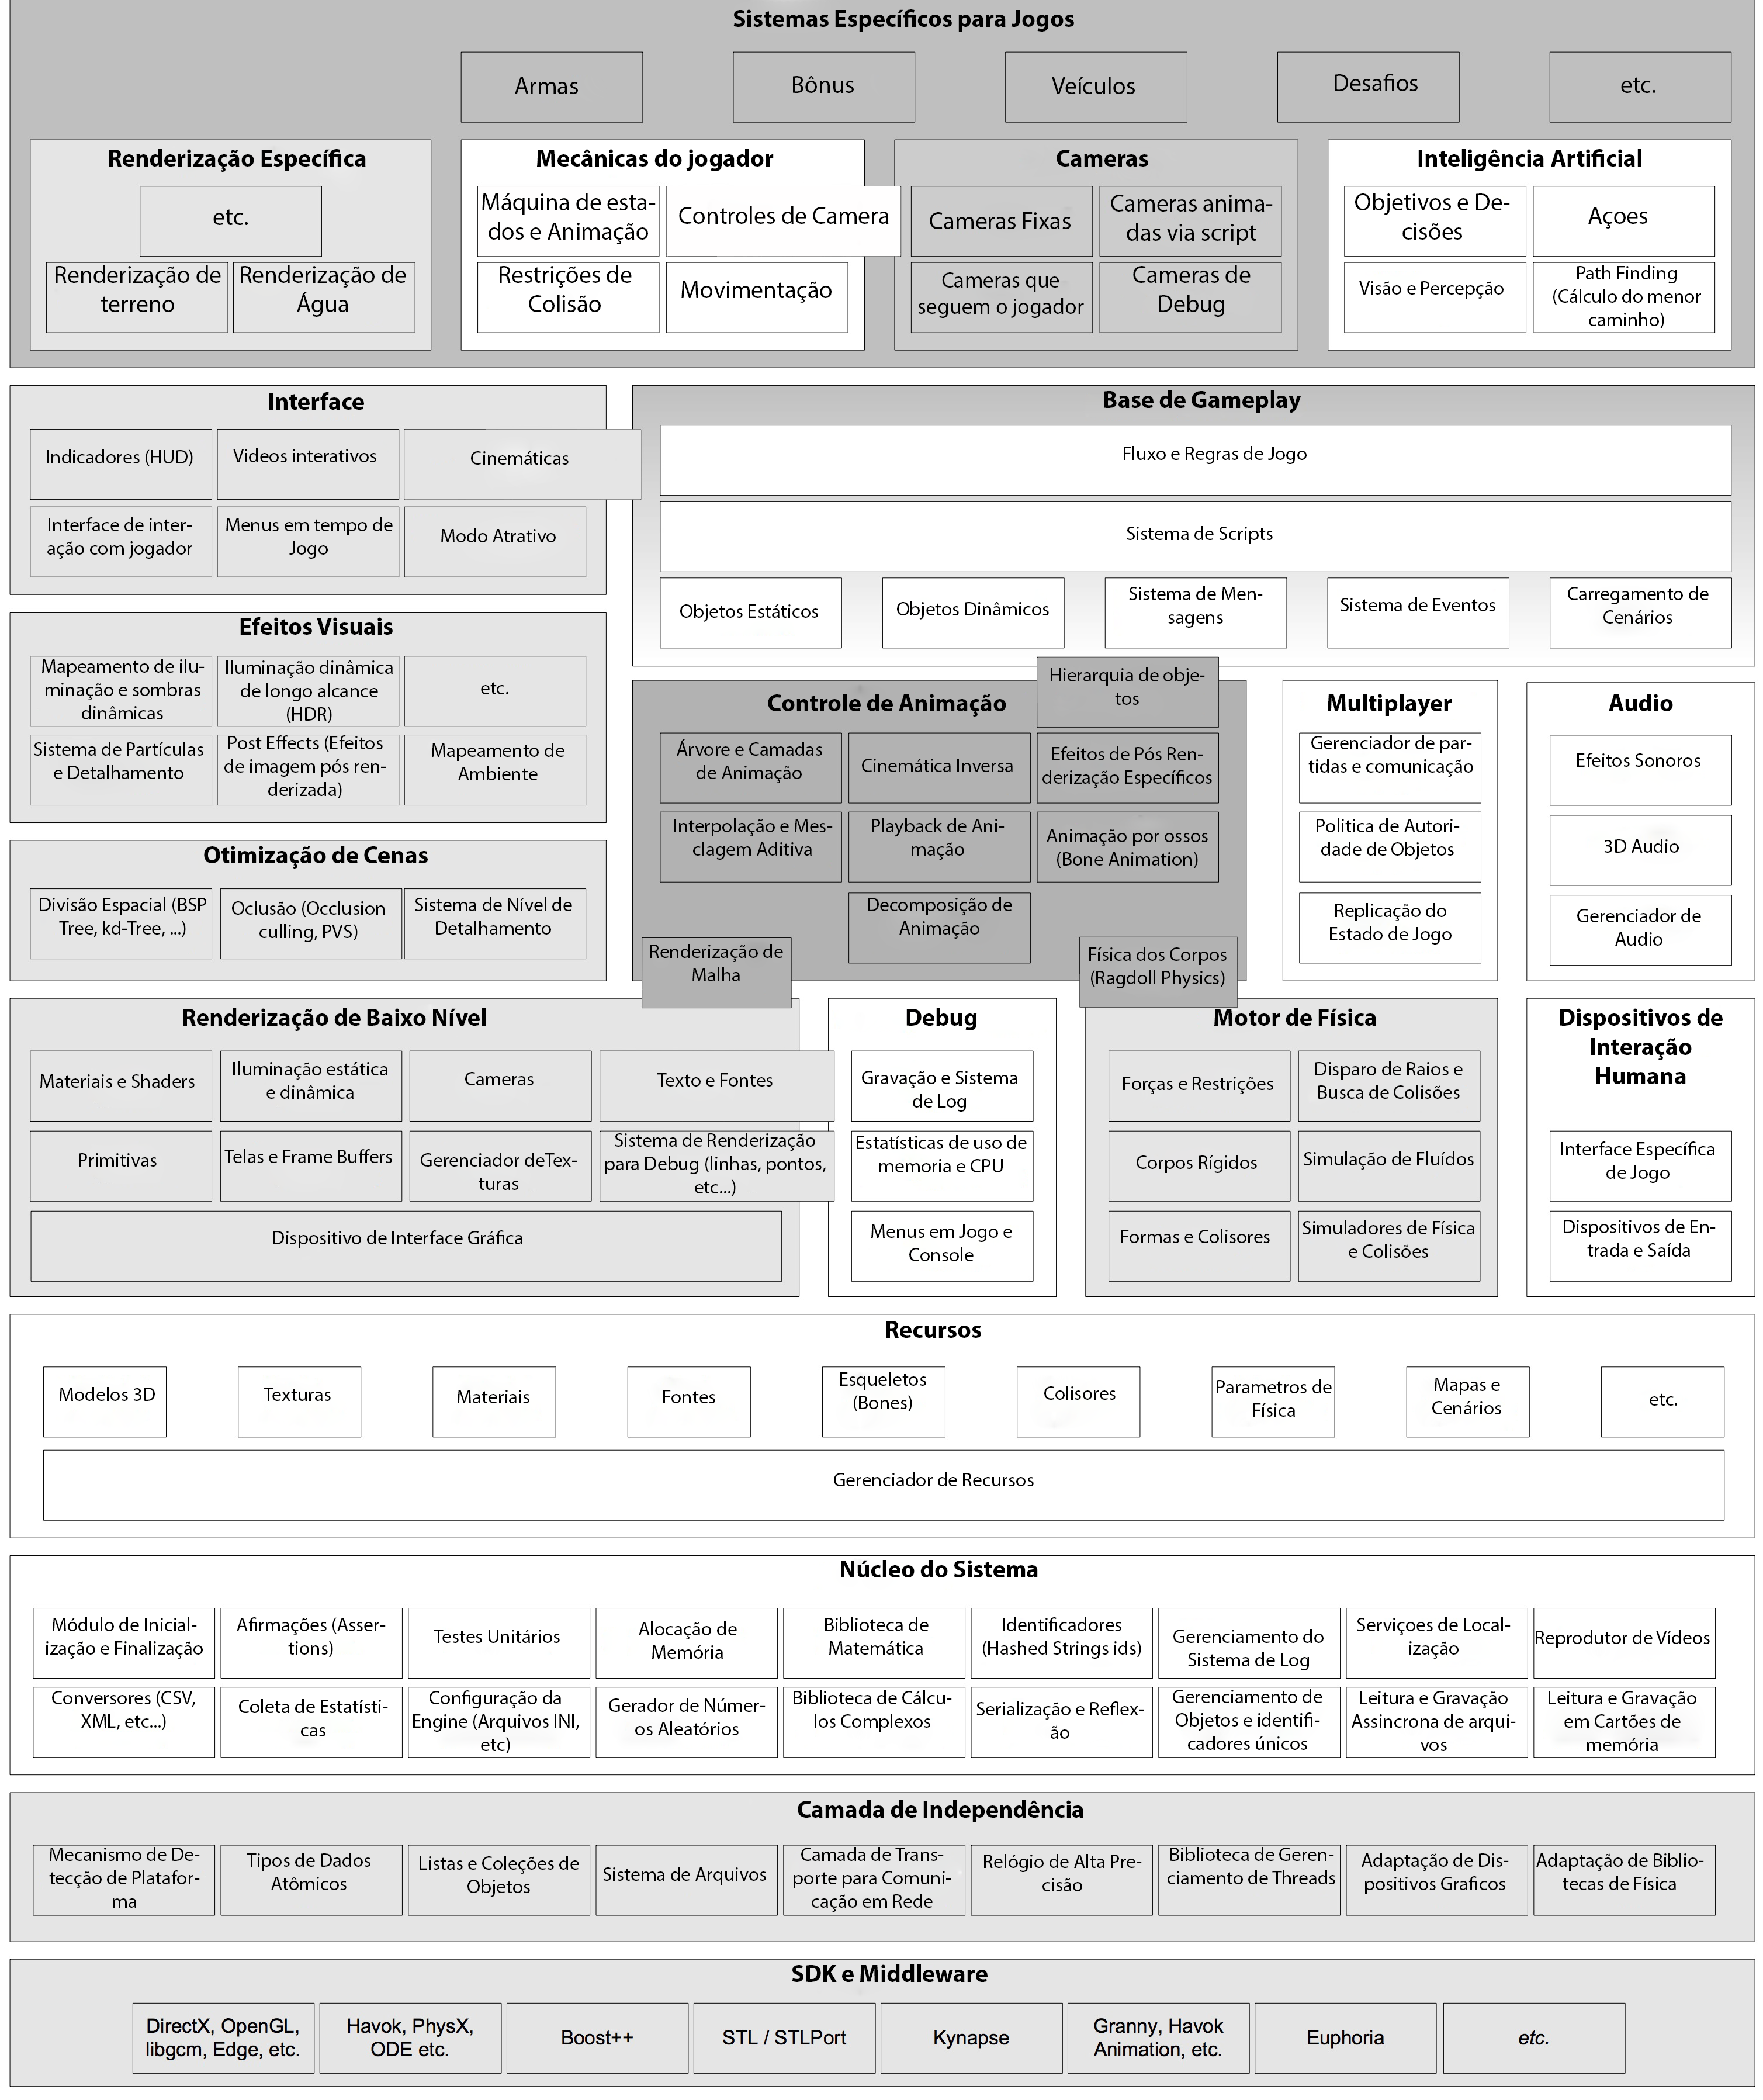
\includegraphics[width=17cm]{imagens/arch.png}
\\
\small{Fonte: Game engine architecture (2011, Página 29)}
\label{figura:arch}
\end{figure}

\subsection{SDK e Middleware}
\textit{SDK e middlewares} são bibliotecas que fornecem abstrações dos recursos de hardware ou software que serão utilizados pela aplicação, a maioria das game engines utilizam essas bibliotecas afim de agilizar e facilitar o desenvolvimento. Nessas bibliotecas podem estar  incluídos algoritmos de inteligência artificial, acesso e manipulação de dispositivos de IO e gráficos, estruturas de dados, cálculos de complexos de física e outros componentes conforme ilustrado na figura \ref{figura:arch_sdk}.

\begin{figure}[H]
\centering
\caption{SDK e middleware}
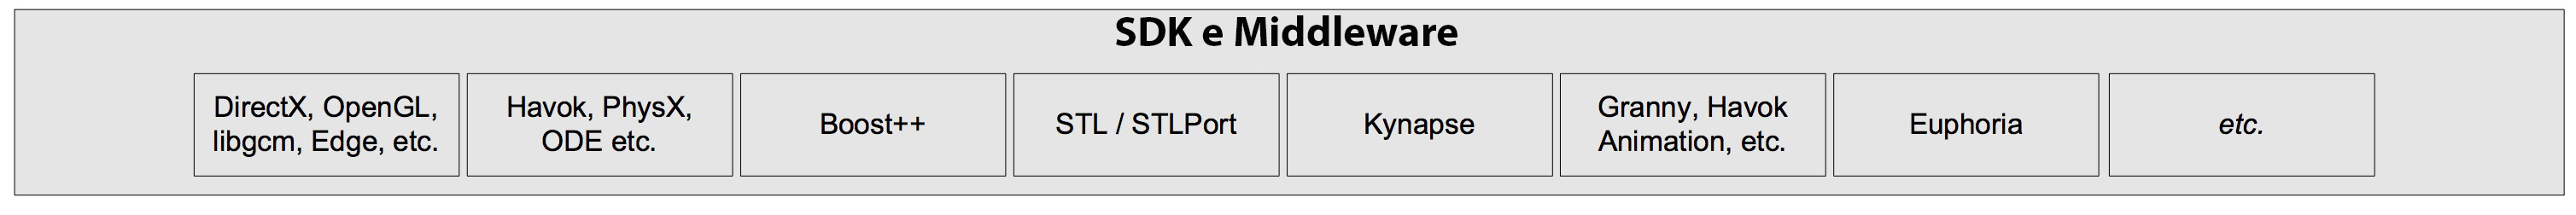
\includegraphics[width=16cm]{imagens/arch-sdk.png}
\\
\small{Fonte: Game engine architecture (2011, Página 29)}
\label{figura:arch_sdk}
\end{figure}

\subsection{Camada de Independência}
A maioria das \textit{game engines} necessitam ser executadas em diferentes plataformas, tanto em hardware como em software, para que isso seja possível é adicionada uma camada de independência, conforme ilustrada na figura \ref{figura:arch_layer}. Esta camada garante que a engine tenha o mesmo comportamento em todas as plataformas.

\begin{figure}[H]
\centering
\caption{Camada de independência}
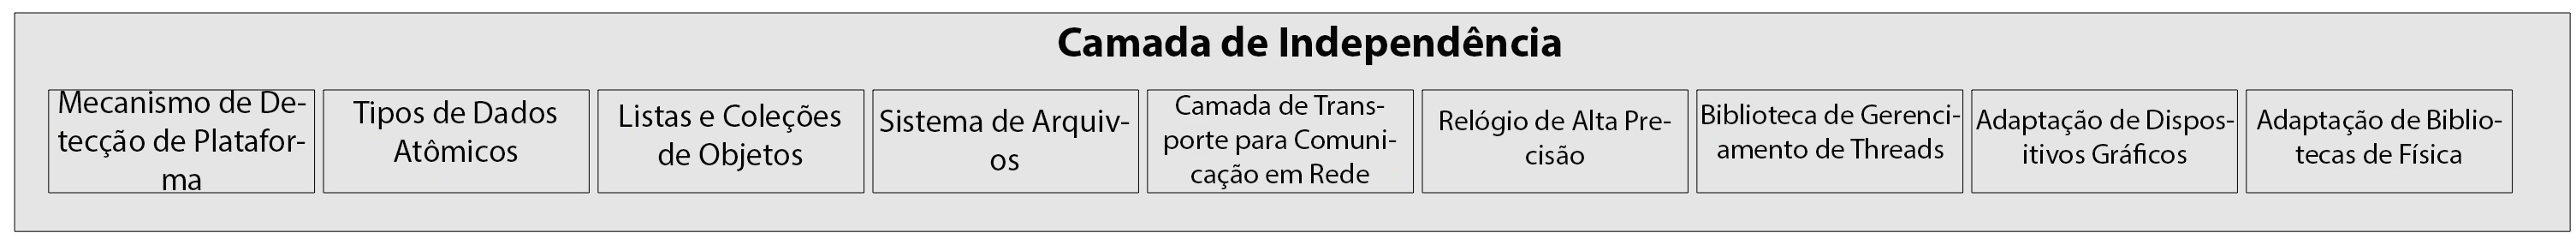
\includegraphics[width=16cm]{imagens/arch-layer.png}
\\
\small{Fonte: Game engine architecture (2011, Página 29)}
\label{figura:arch_layer}
\end{figure}

\subsection{Núcleo do Sistema}
As \textit{game engines}, assim com qualquer outro software, necessitam de um conjunto de ferramentas que sirvam de base para as outras partes do sistema, nas \textit{game engines} estas ferramentas ficam localizadas no núcleo do sistema tambem conhecido como \textit{Core Engine}. No núcleo são definidas as estruturas de dados que não são fornecidas pelos \textit{middlewares}, algoritmos de gerenciamento de memória customizados, bibliotecas que efetuam cálculos matemáticos complexos e algoritmos que auxiliam no \textit{debug} e \textit{log} da aplicação. \\
O núcleo também pode ser responsável pela inicialização e finalização de outros subsistemas, controlar o loop principal de eventos e sincronização de processos adicionais. A figura \ref{figura:arch_core} ilustra alguns componentes presentes nesta camada.

\begin{figure}[H]
\centering
\caption{Núcleo do Sistema}
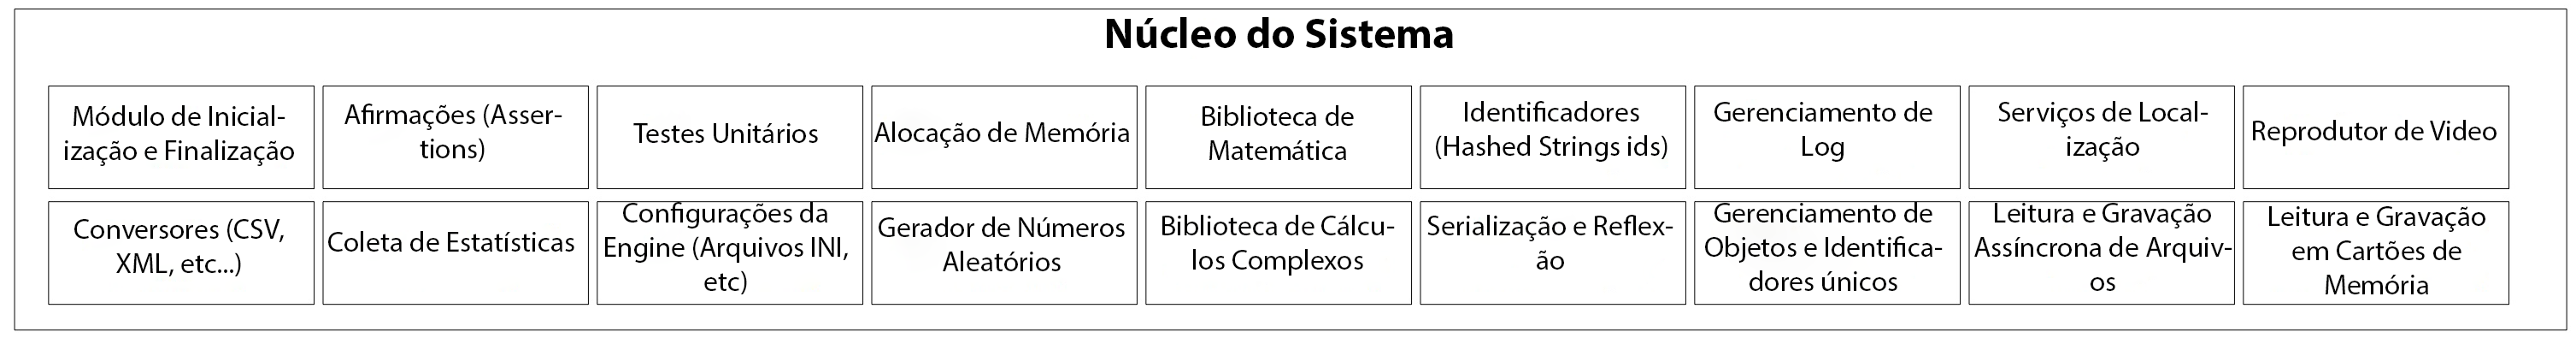
\includegraphics[width=16cm]{imagens/arch-core.png}
\\
\small{Fonte: Game engine architecture (2011, Página 29)}
\label{figura:arch_core}
\end{figure}

\subsection{Gerenciador de Recursos}
Toda \textit{game engine} inclui um sistema de gerenciamento de recursos (ilustrado na figura \ref{figura:arch_res}) que é utilizado para padronizar a forma de acesso aos dados externos que necessitam ser incluídos no jogo (com modelos, texturas, \textit{shader}, etc) e controlar o carregamento, liberação e reutilização desses recursos durante a execução.

\begin{figure}[H]
\centering
\caption{Gerenciador de Recursos}
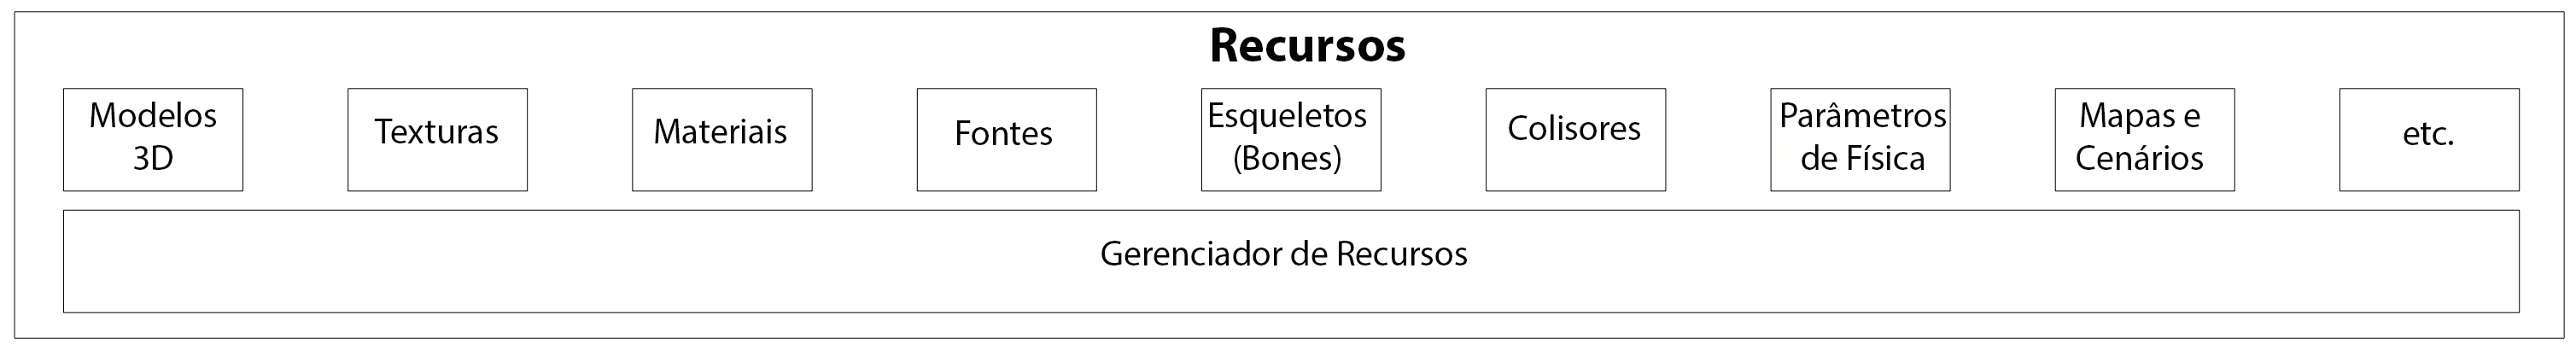
\includegraphics[width=16cm]{imagens/arch-res.png}
\\
\small{Fonte: Game engine architecture (2011, Página 29)}
\label{figura:arch_res}
\end{figure}

\subsection{Motor de Renderização}
O motor renderização (ou \textit{rendering engine}) é a camada da \textit{game engine} responsável pelo acesso e manipulação dos recursos gráficos utilizados pelos jogos. Para a manipulação desses recursos são utilizadas bibliotecas de baixo nível (geralmente implementadas em linguagem C ou C++) que fornecem recursos para a total customização dos aspectos do jogo. O motor de renderização é a maior, mais complexa e mais importante parte da \textit{game engine}, e pode ser dividida em várias camadas.

\subsubsection{Renderização de Baixo Nível}
A renderização de baixo nível (ilustrada na figura \ref{figura:arch-low}) é a camada responsável pela renderização de primitivas básicas (geralmente são utilizados triângulos), alocação e configuração de buffers e cálculos de coloração dos pixels. É nesta camada que são feitas as chamadas às bibliotecas que manipulam os dispositivos gráficos como OpenGL e Direct3D.

\begin{figure}[H]
\centering
\caption{Motor de Renderização - renderização de baixo nível}
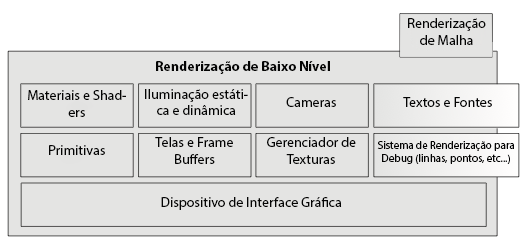
\includegraphics[width=12cm]{imagens/arch-low.png}
\\
\small{Fonte: Game engine architecture (2011, Página 29)}
\label{figura:arch-low}
\end{figure}

\subsubsection{OpenGL e Direct3D}
OpenGL é uma biblioteca desenvolvida em C que fornece acesso aos recursos gráficos de vários tipos de dispositivos, podendo ser implementado em hardware (como placas de video) ou em software caso não exista um hardware gráfico. \cite{shreiner}\\
OpenGL é uma das bibliotecas mais utilizadas no desenvolvimento de jogos pelo fato de ser portável para várias plataformas e por prover acesso e controle de baixo nível ao hardware mesmo em linguagens de nível mais alto como Java e Python.\\
Segundo \citeonline{sellers} esse nível de acesso ao hardware da uma vantagem muito grande a OpenGL em relação a outras API pois permite não só re-implementar as técnicas de renderização já utilizadas, mas também fornece liberdade para que o desenvolvedor teste e invente novas técnicas. OpenGL possui uma sintaxe de programação própria chamada GLSL (\textit{OpenGL Shading Language}) para a produção e controle de efeitos e renderização de imagens.
\\
Direct3D é uma parte da API DirectX voltada para a renderização de gráficos 2D e 3D nas plataformas da Microsoft. Apesar de também fornecer acesso de baixo nível aos recursos de hardware, Direct3D é fortemente orientado a objetos, o que torna o desenvolvimento e a integração com linguagens de alto nível um pouco mais simples. Assim como OpenGL, Direct3D também possui a sua própria sintaxe de programação chamada HLSL (\textit{High Level Shading Language}) e é a linguagem mais utilizada dentro das plataformas da Microsoft devido ao seu desempenho otimizado. Ao contrario de OpenGL, Direct3D contem embutido em sua biblioteca um mecanismo nativo de criação de janelas e captura de inputs chamado XInput e não é portável para outras plataformas.
\\
Tanto OpenGL quando Direct3D fornecem duas formas básicas de renderização, através de um \textit{pipeline} fixo, também conhecido como \textit{Legacy Mode} (Modo Legado) e um \textit{pipeline} programável utilizando \textit{shaders}.

\begin{itemize}
\item \textit{Pipeline} fixo: Consiste em uma serie de etapas necessárias para que o dispositivo gráfico consiga renderizar as imagens desejadas. Estas etapas consistem na especificação dos vértices e primitivas, transformações geométricas, iluminação, rasterização e renderização. Por se tratar de uma rotina fixa, a quantidade de efeitos que podem ser aplicados na imagem final é bastante limitada.
\item \textit{Pipeline} programável: Consiste no mesmo processo que o \textit{pipeline} fixo, mas permite um controle mais fino por parte do programador, já que permite alterações em sua saída através de \textit{shaders} específicos.
\end{itemize}

\textit{Shaders} são programas que são executados internamente nos dispositivos gráficos para manipular os resultados de saída do \textit{pipeline} de renderização. Os \textit{shader} são divididos em três grupos:

\begin{itemize}
\item \textit{Vertex Shader}: O \textit{Vertex Shader} tem por responsabilidade substituir o processo de manipulação dos vértices presente no \textit{pipeline} fixo, permitindo ao programador manipular as transformações geométricas, o posicionamento e cor dos vértices, bem como o processo de iluminação e geração de coordenas de textura na parte dos vértices.
\item \textit{Geometry Shader}: O \textit{Geometry Shader} é um recurso opcional no \textit{pipeline} programável. Sua principal função é a de criar ou remover vértices, permitindo um maior controle na geometria que passa pelo \textit{pipeline} programável, aumentando ou diminuindo o nível de detalhe conforme necessário, permitindo com que uma enorme variedade de efeitos sejam possíveis, como melhor interpolação de vértices com a adição de novos vértices quando necessário, renderização de silhueta, entre outros.
\item \textit{Fragment Shader} (ou \textit{Pixel Shader}): O \textit{Fragment Shader} (ou \textit{Pixel Shader}) tem a função de manipular a coloração dos pixels, calcular a iluminação e manipular as texturas.
\end{itemize}

\subsubsection{Otimização de Cenas}
A camada de Otimização (ilustrada na figura \ref{figura:arch_scene}) é a camada responsável pela remoção de objetos que estão muito distantes, localizados atras da câmera ou escondidos atras de outros objetos da lista de renderização, podendo aumentar drasticamente a performance da aplicação.

\begin{figure}[H]
\centering
\caption{Motor de Renderização - Scene Graph e Culling Optimization}
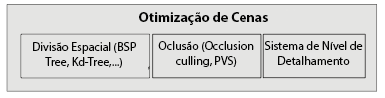
\includegraphics[width=10cm]{imagens/arch-scene.png}
\\
\small{Fonte: Game engine architecture (2011, Página 29)}
\label{figura:arch_scene}
\end{figure}

\subsubsection{Efeitos Visuais}
As \textit{game engines} mais modernas suportam um grande numero de efeitos visuais (conforme ilustrado na figura \ref{figura:arch-visual}). Esses efeitos variam de acordo com o tipo de jogo e a plataforma alvo, geralmente é nesta camada onde são realizados os cálculos mais complexos e pesados da engine.

\begin{figure}[H]
\centering
\caption{Motor de Renderização - Efeitos Visuais}
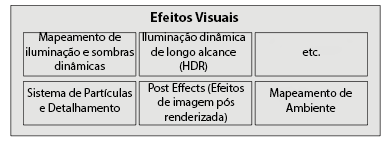
\includegraphics[width=10cm]{imagens/arch-visual.png}
\\
\small{Fonte: Game engine architecture (2011, Página 29)}
\label{figura:arch-visual}
\end{figure}

\subsubsection{Interação com o Usuário}
A maioria dos jogos necessitam de uma interface 2D para a interação com o usuário, seja em um menu de opções ou para exibir a pontuação. A camada de interação com o usuário (ilustrada na figura \ref{figura:arch_front}) é responsável por apresentar essas informações independente da técnica de renderização utilizada.

\begin{figure}[H]
\centering
\caption{Motor de Renderização - Interface com o Usuário}
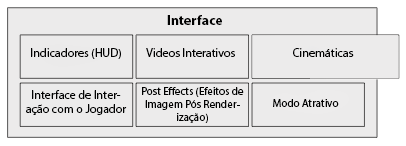
\includegraphics[width=10cm]{imagens/arch-front.png}
\\
\small{Fonte: Game engine architecture (2011, Página 29)}
\label{figura:arch_front}
\end{figure}

\subsection{Motor de Física}
O motor de física é uma das camadas indispensáveis em uma \textit{game engine}, pois é ela que provê um comportamento realista ao jogo. A maioria dos motores de física consiste em um mecanismo detector de colisões, um sistema de simulação de corpos rígidos e fluidos, podendo eles serem baseados nas regras do mundo real ou não. A figura \ref{figura:arch_phys} mostra alguns componentes presentes nesta camada.

\begin{figure}[H]
\centering
\caption{Motor de Física}
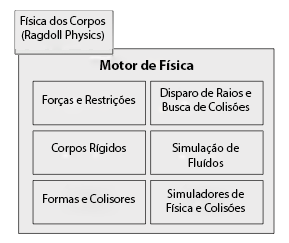
\includegraphics[width=7cm]{imagens/arch-phys.png}
\\
\small{Fonte: Game engine architecture, 2011}
\label{figura:arch_phys}
\end{figure}

\subsection{Dispositivos de Interação Humana}
A camada de dispositivos de interação humana (ilustrado na figura \ref{figura:arch_hid}) é responsável por capturar, processar e redirecionar as entradas do usuário para as demais áreas da engine. Estas entradas podem ser feitas através do teclado, mouse, \textit{joystick} ou qualquer outro dispositivo conectado ao hardware onde será executado o jogo.

\begin{figure}[H]
\centering
\caption{Dispositivos de Interação Humana}
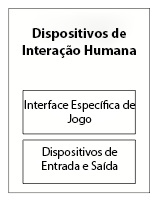
\includegraphics[width=5cm]{imagens/arch-hid.png}
\\
\small{Fonte: Game engine architecture (2011, Página 29)}
\label{figura:arch_hid}
\end{figure}

\subsection{Motor de Áudio}
O motor de áudio (figura \ref{figura:arch_audio}) é a camada responsável por acessar e manipular os recurso de áudio utilizados pelos jogos. Geralmente são utilizadas bibliotecas de baixo nível desenvolvidas em C que são capazes se simular áudios em 2D e 3D. AS API`s mais utilizadas são OpenAL e DirectX Audio.

\begin{figure}[H]
\centering
\caption{Motor de Áudio}
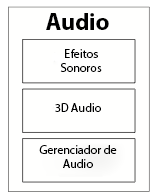
\includegraphics[width=5cm]{imagens/arch-audio.png}
\\
\small{Fonte: Game engine architecture (2011, Página 29)}
\label{figura:arch_audio}
\end{figure}

\subsubsection{OpenAL e DirectX Audio}
OpenAL é uma biblioteca de audio multi-plataforma que possibilita a reprodução de audio em três dimensões, o que a torna ideal para varias aplicações de audio, principalmente para jogos. \cite{hiebert}
\\
DirectX Audio é uma parte da API DirectX que combina duas bibliotecas DirectSound e DirectMusic, onde uma é utilizada para efeitos sonoros e a outra para reprodução de áudio em alta qualidade.

\subsection{Motor de Comunicação em Rede}
O motor de comunicação em rede (ilustrado na figura \ref{figura:arch_network}) é uma camada opcional que permite a troca de informações entre duas instâncias do mesmo jogo. Devido a complexidade de implementar a troca de informações em alta velocidade sem afetar performance dos jogos, esta camada é implementada somente em jogos que necessitam desse tipo de comunicação.

\begin{figure}[H]
\centering
\caption{Motor de Comunicação em Rede}
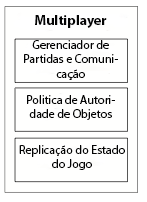
\includegraphics[width=5cm]{imagens/arch-network.png}
\\
\small{Fonte: Game engine architecture (2011, Página 29)}
\label{figura:arch_network}
\end{figure}

\subsection{Base de Gameplay}
A Base de gameplay (ilustrada na figura \ref{figura:arch_gameplay}) é uma camada responsável pela lógica executada em tempo de jogo e base para a criação de objetos. A organização desses objetos varia de acordo com a necessidade, mas na maioria dos casos os objetos são organizados em cenas, onde cada cena pode ser uma fase ou uma sala especifica dentro do jogo. A hierarquia dos objetos dentro da cena pode ser feita de duas maneiras, através de um sistema de herança ou baseado em componentes.

\begin{figure}[H]
\centering
\caption{Base de Gameplay}
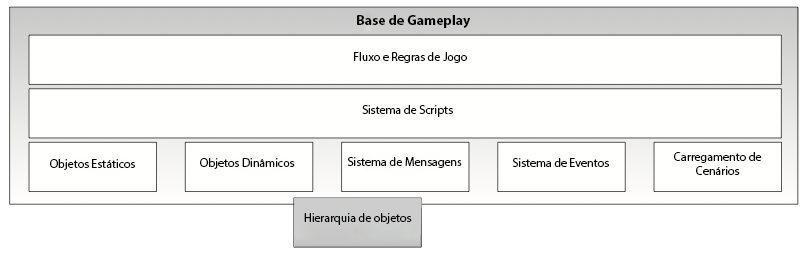
\includegraphics[width=17cm]{imagens/arch-gameplay.png}
\\
\small{Fonte: Game engine architecture (2011, Página 29)}
\label{figura:arch_gameplay}
\end{figure}

\begin{itemize}
\item Sistema baseado em herança: É criada uma herança de classes, onde cada objeto tem o seu comportamento definido pelas funções implementadas nele e em seus predecessores. (figura \ref{figura:arch_heranca})
\end{itemize}

\begin{figure}[H]
\centering
\caption{Base de Gameplay - arquitetura baseada em herança}
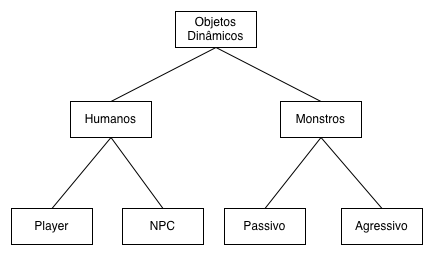
\includegraphics[width=10cm]{imagens/arch-heranca.png}
\\
\small{Fonte: Elaborado pelo autor}
\label{figura:arch_heranca}
\end{figure}

\begin{itemize}
\item Sistema baseado em componentes: Cada objeto funciona como um conteiner, onde os componentes adicionados a ele definem o seu comportamento e atributos.(figura \ref{figura:arch_comp})
\end{itemize}

\begin{figure}[H]
\centering
\caption{Base de Gameplay - arquitetura baseada em componentes}
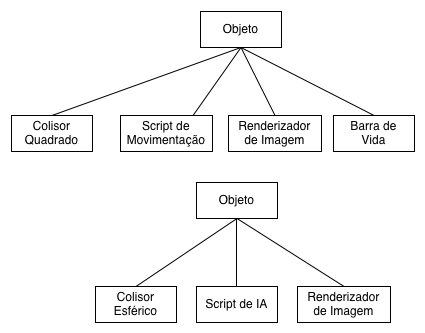
\includegraphics[width=10cm]{imagens/arch-comp.png}
\\
\small{Fonte: Elaborado pelo autor}
\label{figura:arch_comp}
\end{figure}

Geralmente esta camada inclui um motor de manipulação de \textit{scripts} que funciona como uma maquina virtual que interpreta \textit{scripts} desenvolvidos em uma linguagem diferente do resto da \textit{engine}, a fim de oferecer flexibilidade, facilidade e velocidade de execução. Praticamente qualquer linguagem pode ser implementada na \textit{scripting engine}, as mais utilizadas são LUA, JavaScript, Python e C\#.

\subsection{Sistemas Específicos para Jogos}
O objetivo principal de uma \textit{game engine} é fornecer um conjunto básico de funcionalidades que são comuns na maioria dos jogos, acima de todas as camadas anteriores são construídos os sistemas únicos para cada jogo. Nesta camada são definidos os modelos, as texturas e toda a lógica implementada para um jogo, conforme ilustrado na figura \ref{figura:arch_game}.

\begin{figure}[H]
\centering
\caption{Sistemas Específicos para Jogos}
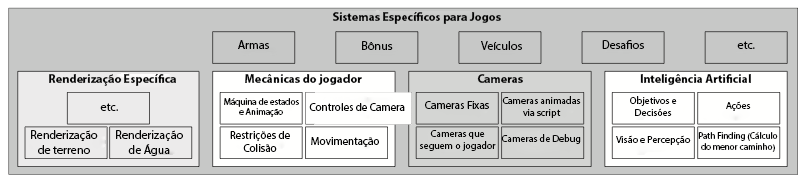
\includegraphics[width=17cm]{imagens/arch-game.png}
\\
\small{Fonte: Game engine architecture (2011, Página 29)}
\label{figura:arch_game}
\end{figure}

%%%%%%%%%%%%%%%%%%%%%%%%%%%%%%%%%%%%%%%%%%%%%%%%%
%
%		Finalização
%
%%%%%%%%%%%%%%%%%%%%%%%%%%%%%%%%%%%%%%%%%%%%%%%%%

Com a arquitetura em camadas é possível adicionar e remover funcionalidades sem que seja necessário rescrever todo o software. Para que esta arquitetura funcione cada camada deve ter apenas uma função e deve ser ligada a uma das camadas essenciais para o funcionamento da \textit{engine}. Uma \textit{game engine} pode ser implementada com praticamente qualquer linguagem, tendo ela acesso nativo ao hardware ou não, caso a linguagem não tenha acesso ao hardware, o controle pode ser feito via software (geralmente fazendo chamadas ao sistema operacional ou a algum outro software que tenha acesso direto), impossibilitando o controle completo das camadas de nível mais baixo por parte do desenvolvedor. \\
No capítulo \ref{cap: desenvolvimento} estão descritas as ferramentas e técnicas utilizadas no desenvolvimento da Pulsar Game Engine.


%%%%%%%%%%%%%%%%%%%%%%%%%%%%%%%%%%%%%%%%%%%%%%%%%
%
%		Desenvolvimento
%
%%%%%%%%%%%%%%%%%%%%%%%%%%%%%%%%%%%%%%%%%%%%%%%%%

\chapter{Pulsar Game Engine} \label{cap: desenvolvimento}

%%%%%%%%%%%%%%%%%%%%%%
%
%		Projeto
%
%%%%%%%%%%%%%%%%%%%%%%

\section{Projeto}

As tecnologias utilizadas nesse projeto foram escolhidas visando a maior portabilidade possível sem que fosse necessário recompilar a \textit{engine}, para isso foram escolhidas as linguagens Java e JavaScript para o desenvolvimento do núcleo e dos \textit{scripts} executados durante o jogo. Devido a complexidade do projeto algumas bibliotecas auxiliares foram escolhidas para agilizar o desenvolvimento, para controle sobre o hardware gráfico e som foi escolhido uma adaptação das bibliotecas OpenGL e OpenAL para Java chamada LWJGL (\textit{Lightweight Java Game Library}), para as simulações de física em duas dimensões foi escolhida a biblioteca Box2D e para compilação e gerenciamento das dependencias foi utilizado Gradle. \\
A \textit{game engine} recebeu o nome de Pulsar Game Engine e seu código fonte está disponível no link \textit{https://github.com/Netoaoh/pulsar-game-engine} sob a licença GPL-3.0.

%%%%%%%%%%%%%%%%%%%%%%
%
%		Arquitetura
%
%%%%%%%%%%%%%%%%%%%%%%

\section{Arquitetura}

A Pulsar Game Engine possui uma arquitetura baseada em \textit{Game Objects} e \textit{Game Components}, onde os \textit{Game Objects} funcionam como containers e os \textit{Game Components} definem as propriedades e o comportamento desses objetos dentro do jogo, com isso é possível criar uma variação grande de objetos utilizando o mesmo código. \\
Para facilitar a extensão e customização da \textit{engine}, todos os sub-sistemas são implementados em cima de classes abstratas, que definem os métodos principais para o funcionamento correto da \textit{engine}. Essas classes possuem o prefixo "I" seguido do nome do sub-sistema (figura \ref{figura:subengine-interface}) e são instanciados e registrados antes da inicialização do \textit{loop} principal (figura \ref{figura:codigo-main}), desta forma é possivel alterar o comportamento da engine sem que seja necessário alterar a biblioteca principal.

\begin{figure}[H]
\centering
\caption{Classe base de sub-sistema}
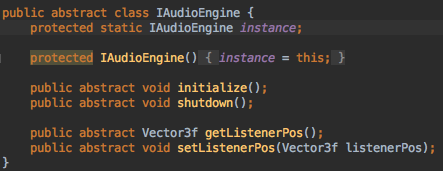
\includegraphics[width=12cm]{imagens/subengine-interface.png}
\\
\small{Fonte: Elaborado pelo autor}
\label{figura:subengine-interface}
\end{figure}

\begin{figure}[H]
\centering
\caption{Código da classe principal}
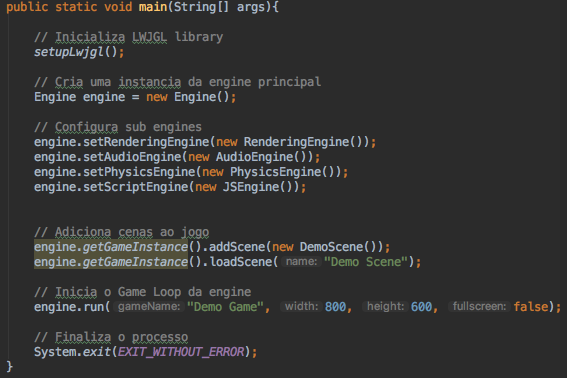
\includegraphics[width=12cm]{imagens/codigo-main.png}
\\
\small{Fonte: Elaborado pelo autor}
\label{figura:codigo-main}
\end{figure}

%%%%%%%%%%%%%%%%%%%%%%
%
%		Componentes
%
%%%%%%%%%%%%%%%%%%%%%%

\section{Componentes}

Componentes ou \textit{Game Components} são classes que definem as propriedades e o comportamento dos objetos em jogo, cada \textit{Game Object} pode conter um ou mais componentes. \\
Cada Componente possui um ou mais metodos que são executados em momentos específicos do fluxo de execução da \textit{engine}. Esses métodos são:

\begin{itemize}
\item \textit{Awake}: Executado quando o componente é adicionado ao \textit{Game Object}.
\item \textit{Start}: Executado quando a cena é carregada e exibida.
\item \textit{Update}: Executado a cada iteração do fluxo de execução.
\item \textit{FixedUpdate}: Executado a cada iteração da engine de física (30 vezes por segundo).
\item \textit{Render}: Executado 60 vezes por segundo.
\item \textit{OnCollisionEnter}: Executado quando há uma colisão entre dois ou mais objetos.
\end{itemize}

Os componentes disponíveis por padrão na Pulsar Game Engine são:

\begin{itemize}
\item \textit{AnimationComponent}: Componente utilizado para controlar animações de \textit{sprites}. 
\item \textit{AudioListenerComponent}: Componente utilizado como receptor de som dentro da \textit{engine}.
\item \textit{AudioSourceComponent}: Componente utilizado como fonte de som dentro da \textit{engine}.
\item \textit{BoxCollider}: Componente que define e controla a caixa de colisão de um objeto.
\item \textit{Camera}: Componente que define a posição e as propriedade de visão dentro da \textit{engine}.
\item \textit{ScriptComponent}: Componente que provê controle sobre a lógica de um objeto em tempo de execução.
\item \textit{SpriteRenderer}: Componente que possibilita a renderização de um \textit{sprite}.
\item \textit{Transform}: Componente que armazena as informações de posição, rotação e escala de um objeto (este componente é padrão e obrigatório para todos os objetos em cena).
\end{itemize}

Novos componentes podem ser criados e integrados a \textit{engine} estendendo a classe \textit{Component}.

%%%%%%%%%%%%%%%%%%%%%%
%
%		Lógica em tempo de jogo
%
%%%%%%%%%%%%%%%%%%%%%%

\section{Lógica em tempo de jogo}

Para controlar a lógica executada durante o jogo a Pulsar Game Engine possui um sistema de \textit{scripts} que interpreta a linguagem JavaScript em tempo de execução utilizando o motor ja imbutido na linguagem Java. \\
O sistema de script expõe os métodos \textit{Awake}, \textit{Start}, \textit{Update}, \textit{FixedUpdate} e \textit{OnCollisionEnter} para serem manipulados no \textit{script}.

%%%%%%%%%%%%%%%%%%%%%%
%
%		Técnicas de Renderização
%
%%%%%%%%%%%%%%%%%%%%%%

\section{Técnicas de Renderização}

Com a utilização dos \textit{shaders} é possível implementar diversas técnicas de renderização, para este projeto foi escolhida a técnica \textit{multi-pass forward rendering}, que consiste em renderizar os objetos várias vezes aplicando diferentes \textit{shaders} (um shader para cada efeito ou ponto de luz presente na cena) e posteriormente combinando as imagens utilizando a técnica de mesclagem aditiva (\textit{Additive Blending}) para formar a imagem final. Esta técnica foi escolhida devido a facilidade de implementação e a performance superior em cenas simples comparado a outras técnicas.

%%%%%%%%%%%%%%%%%%%%%%
%
%		Fluxo de Execução
%
%%%%%%%%%%%%%%%%%%%%%%

\section{Fluxo de Execução}
Esta seção apresenta o fluxo de execução da engine em desenvolvimento (figura \ref{figura:gameloop})

\begin{figure}[H]
\centering
\caption{Loop principal}
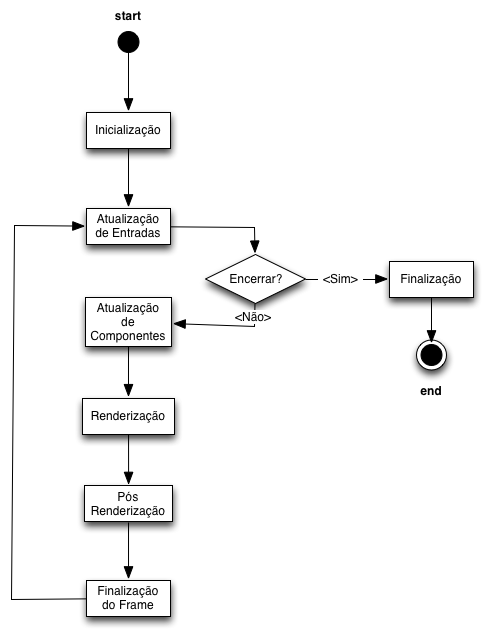
\includegraphics[width=12cm]{imagens/gameloop.png}
\\
\small{Fonte: Elaborado pelo autor}
\label{figura:gameloop}
\end{figure}

\subsection{Inicialização}
Na inicialização do sistema são carregadas todas as configurações e inicializados todos os subsistemas necessários para que o jogo funcione corretamente, é nesta etapa que são criados os \textit{framebuffers} e carregadas as definições das cenas.

\subsection{Atualização de entradas}
Nesta etapa do loop principal são capturadas e armazenadas as entradas do usuário para serem utilizadas por qualquer componente que necessite dessas informações. Nesta etapa também é feita uma verificação para que o jogo seja finalizado ou não, saindo assim do loop infinito.

\subsection{Atualização de componentes}
Nessa etapa todos os componentes de todos os objetos instanciados na cena são atualizados, conforme ilustrado na figura \ref{figura:update}. Cada componente é enviado e armazenado temporariamente no subsistema que é responsável pela sua execução, este subsistema realiza a atualização dos componentes e limpa a sua lista interna de atualização. \\
Por questões de performance os componentes de renderização são agrupados em lotes (\textit{batches}) que são enviados para o motor de renderização, onde serão renderizados de acordo com esses grupos, conforme descrito na seção \ref{sec: renderizacao}.

\begin{figure}[H]
\centering
\caption{Ciclo de atualização dos componentes}
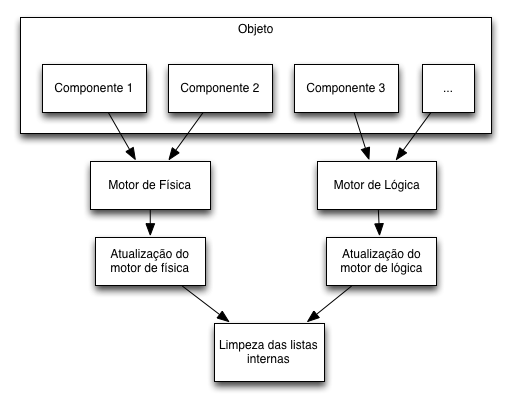
\includegraphics[width=12cm]{imagens/update.png}
\\
\small{Fonte: Elaborado pelo autor}
\label{figura:update}
\end{figure}

\subsection{Renderização}  \label{sec: renderizacao}
Na etapa de renderização os dados dos objetos agrupados são enviados para os \textit{buffers} da placa de video e renderizados na tela conforme ilustrado na figura \ref{figura:render}.

\begin{figure}[H]
\centering
\caption{Ciclo de renderização dos componentes}
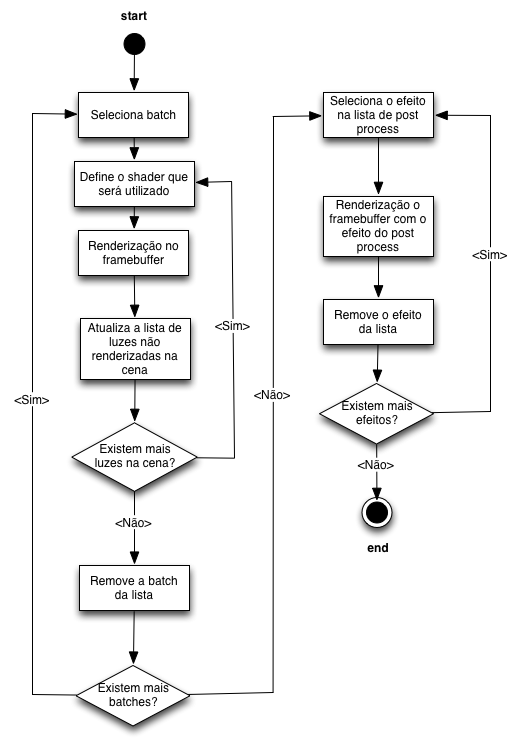
\includegraphics[width=12cm]{imagens/render.png}
\\
\small{Fonte: Elaborado pelo autor}
\label{figura:render}
\end{figure}

\subsection{Pós Renderização}
A etapa de pós renderização é utilizada para atualizações que necessitam ser feitas após os objetos serem renderizados na tela (como a movimentação da câmera por exemplo), afim de prevenir erros de renderização.

\subsection{Finalização do Frame}
Etapa que finaliza o frame limpado os \textit{buffers} de renderização da janela e liberando recursos que não serão reutilizados no próximo frame (como objetos e componentes removidos da cena).

\subsection{Finalização da Engine}
Caso seja enviado um comando de finalização todos os recursos alocados pela engine são liberados, garantindo a finalização do programa de maneira segura e sem desperdício de memória (\textit{memory leaks}). 


%%%%%%%%%%%%%%%%%%%%%%
%
%		Utilização
%
%%%%%%%%%%%%%%%%%%%%%%

\section{Utilização}

A Pulsar Game Engine foi desenvolvida utilizando a ferramenta \textit{Gradle} para compilar e gerenciar as dependencias do projeto, desta forma para criar um novo jogo utilizando a \textit{engine}, basta utilizar o template disponível nos exemplos do repositório (figura \ref{figura:estrutura-pastas}), definir os objetos iniciais de cada cena disponível no jogo (figura \ref{figura:custom-scene}) e caso necessário estender ou reimplementar os sistemas internos da \textit{engine}. Toda a lógica executada durante o jogo deve ser implementada em \textit{scripts} utilizando a linguagem JavaScript.

\begin{figure}[H]
\centering
\caption{Estrutura de pastas de um projeto utilizando a Pulsar Game Engine}
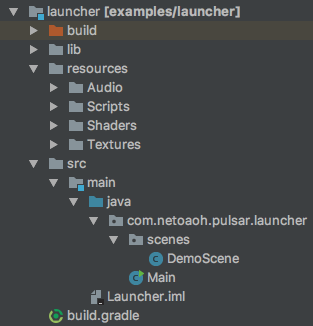
\includegraphics[width=12cm]{imagens/estrutura-pastas.png}
\\
\small{Fonte: Elaborado pelo autor}
\label{figura:estrutura-pastas}
\end{figure}

\begin{figure}[H]
\centering
\caption{Definição de objetos em uma cena}
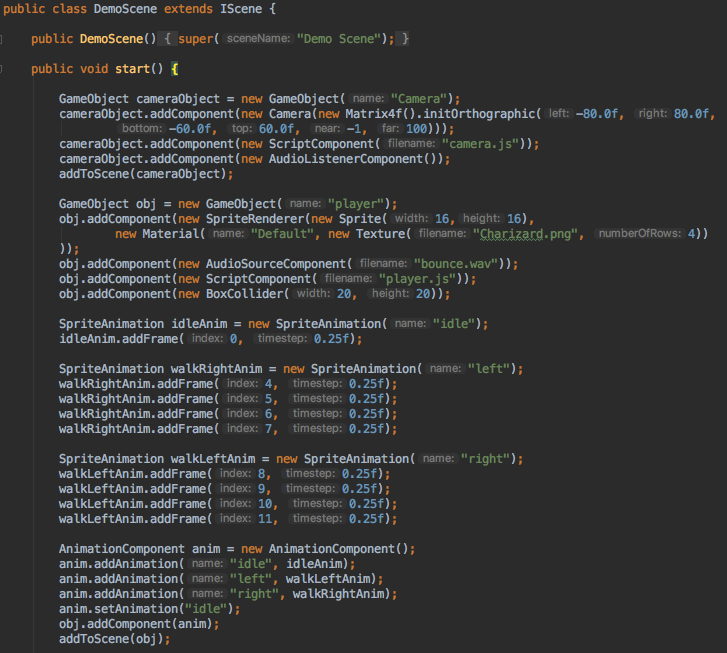
\includegraphics[width=12cm]{imagens/custom-scene.png}
\\
\small{Fonte: Elaborado pelo autor}
\label{figura:custom-scene}
\end{figure}

%%%%%%%%%%%%%%%%%%%%%%%%%%%%%%%%%%%%%%%%%%%%%%%%%
%
%		Conclusão
%
%%%%%%%%%%%%%%%%%%%%%%%%%%%%%%%%%%%%%%%%%%%%%%%%%

\chapter{Conclusão} \label{cap: conclusao}


O Desenvolvimento de uma \textit{game engine} é uma tarefa difícil e trabalhosa que traz muitos benefícios pelo fato de serem implementações abstratas que servem de base para vários jogos, diminuindo assim o custo e o tempo de produção. O fato das \textit{game engines} serem organizadas em camadas facilita a visualização de dependências e customização de seus componentes internos, desta forma pode-se escolher quais camadas implementar de acordo com o objetivo final. A Pulsar Game Engine implementa os componentes básicos necessários para a criação de jogos e uma arquitetura de objetos baseada em componentes, desta forma a customização da \textit{engine} é feita de maneira simples, adicionando componentes e alterando o seu funcionamento conforme a necessidade, resultando em um software polido e enxuto. \\
Apesar de se tratar de uma engine simples, a Pulsar Game Engine consegue produzir jogos de genero variado sem a necessidade de conhecimentos avançados de programação e computação gráfica.


% ----------------------------------------------------------
% Finaliza a parte no bookmark do PDF
% para que se inicie o bookmark na raiz
% e adiciona espaço de parte no Sumário
% ----------------------------------------------------------
\phantompart

% ----------------------------------------------------------
% ELEMENTOS PÓS-TEXTUAIS
% ----------------------------------------------------------
\postextual
% ----------------------------------------------------------

% ----------------------------------------------------------
% Referências bibliográficas
% ----------------------------------------------------------
%\bibliography{abntex2-modelo-references}
\bibliographystyle{abntex2-alf}
\bibliography{referencias}

%---------------------------------------------------------------------
% INDICE REMISSIVO
%---------------------------------------------------------------------
%\phantompart
\printindex
%---------------------------------------------------------------------

\end{document}